\section{Vektorji}

\begin{frame}
    \sectionpage
\end{frame}

\begin{frame}
    \tableofcontents[currentsection, hideothersubsections]
\end{frame}

    \subsection{Vektorske količine}

        \begin{frame}
            \frametitle{Vektorske količine}
        \end{frame}

    \subsection{Računanje z vektorji}

        \begin{frame}
            \frametitle{Računanje z vektorji}
        \end{frame}

    \subsection{Linearna kombinacija vektorjev, baza}

        \begin{frame}
            \frametitle{Koplanarni vektorji}

            \only<2->{\begin{alertblock}{}
                Vektorji so \textbf{koplanarni}, če ležijo na isti ravnini. Rečemo tudi, da so \textbf{linearno odvisni}.
            \end{alertblock}}

            \only<3->{\begin{alertblock}{}
                Če so $\vec{a}$, $\vec{b}$ in $\vec{c}$ koplanarni vektorji, potem velja vsaj ena izmed naslednjih zvez:
                $$\vec{c}=\alpha\vec{a}+\beta\vec{b};\ \alpha,\beta\in\mathbb{R}$$
                $$\vec{b}=\alpha\vec{a}+\gamma\vec{c};\ \alpha,\gamma\in\mathbb{R}$$
                $$\vec{a}=\beta\vec{b}+\gamma\vec{c};\ \beta,\gamma\in\mathbb{R}$$
            \end{alertblock}}

            \only<4->{\begin{alertblock}{}
                Če so vektorji $\vec{a}$, $\vec{b}$ in $\vec{c}$ \textbf{nekoplanarni} oziroma \textbf{linearno neodvisni}, velja: $$\alpha\vec{a}+\beta\vec{b}+\gamma\vec{c}=\vec{0} \Leftrightarrow \alpha =\beta =\gamma =0$$
            \end{alertblock}}
        \end{frame}

        \begin{frame}
            \frametitle{Baza prostora}

            \begin{columns}
                
                \column{0.5\textwidth}
                    \only<2->{\begin{alertblock}{}
                        \textbf{Bazo prostora} tvorijo trije neničelni vektorji ($\vec{a}$, $\vec{b}$, $\vec{c}$), ki ne ležijo na isti ravnini (so nekoplanarni). \\ Imenujemo jih \textbf{bazni vektorji} prostora.
                    \end{alertblock}}

                \column{0.48\textwidth}


                \only<2->{\begin{tikzpicture}
                    % \clip (0,0) rectangle (14.000000,10.000000);
                    {\footnotesize
                    \only<4->{
                    % Drawing segment A B
                    \draw [line width=0.016cm] (1.500000,2.500000) -- (3.500000,1.500000);%
                    
                    % Drawing arrow A B 1.00
                    \draw [line width=0.016cm] (3.251479,1.668040) -- (3.500000,1.500000);%
                    \draw [line width=0.016cm] (3.251479,1.668040) -- (3.411322,1.544339);%
                    \draw [line width=0.016cm] (3.216456,1.597992) -- (3.500000,1.500000);%
                    \draw [line width=0.016cm] (3.216456,1.597992) -- (3.411322,1.544339);%
                    
                    % Drawing segment A C
                    \draw [line width=0.016cm] (1.500000,2.500000) -- (3.000000,3.500000);%
                    
                    % Drawing arrow A C 1.00
                    \draw [line width=0.016cm] (2.730800,3.367595) -- (3.000000,3.500000);%
                    \draw [line width=0.016cm] (2.730800,3.367595) -- (2.917507,3.445005);%
                    \draw [line width=0.016cm] (2.774241,3.302432) -- (3.000000,3.500000);%
                    \draw [line width=0.016cm] (2.774241,3.302432) -- (2.917507,3.445005);%
                    
                    % Drawing segment A D
                    \draw [line width=0.016cm] (1.500000,2.500000) -- (1.000000,4.500000);%
                    
                    % Drawing arrow A D 1.00
                    \draw [line width=0.016cm] (1.034150,4.201950) -- (1.000000,4.500000);%
                    \draw [line width=0.016cm] (1.034150,4.201950) -- (1.024046,4.403816);%
                    \draw [line width=0.016cm] (1.110127,4.220944) -- (1.000000,4.500000);%
                    \draw [line width=0.016cm] (1.110127,4.220944) -- (1.024046,4.403816);%
                    
                    % Drawing segment A E
                    \draw [line width=0.016cm] (1.500000,2.500000) -- (1.649942,2.504165);%
                    \draw [line width=0.016cm] (1.724913,2.506248) -- (1.874855,2.510413);%
                    \draw [line width=0.016cm] (1.949826,2.512495) -- (2.099769,2.516660);%
                    \draw [line width=0.016cm] (2.174740,2.518743) -- (2.324682,2.522908);%
                    \draw [line width=0.016cm] (2.399653,2.524990) -- (2.549595,2.529155);%
                    \draw [line width=0.016cm] (2.624566,2.531238) -- (2.774508,2.535403);%
                    \draw [line width=0.016cm] (2.849479,2.537486) -- (2.999422,2.541651);%
                    \draw [line width=0.016cm] (3.074393,2.543733) -- (3.224335,2.547898);%
                    \draw [line width=0.016cm] (3.299306,2.549981) -- (3.449248,2.554146);%
                    \draw [line width=0.016cm] (3.524219,2.556228) -- (3.674161,2.560393);%
                    \draw [line width=0.016cm] (3.749132,2.562476) -- (3.899075,2.566641);%
                    \draw [line width=0.016cm] (3.974046,2.568723) -- (4.123988,2.572889);%
                    \draw [line width=0.016cm] (4.198959,2.574971) -- (4.348901,2.579136);%
                    \draw [line width=0.016cm] (4.423872,2.581219) -- (4.573814,2.585384);%
                    \draw [line width=0.016cm] (4.648785,2.587466) -- (4.798728,2.591631);%
                    \draw [line width=0.016cm] (4.873699,2.593714) -- (5.023641,2.597879);%
                    \draw [line width=0.016cm] (5.098612,2.599961) -- (5.100000,2.600000);%
                    
                    % Drawing segment B E
                    \draw [line width=0.016cm] (3.500000,1.500000) -- (3.623606,1.584979);%
                    \draw [line width=0.016cm] (3.685409,1.627469) -- (3.809016,1.712448);%
                    \draw [line width=0.016cm] (3.870819,1.754938) -- (3.994425,1.839917);%
                    \draw [line width=0.016cm] (4.056228,1.882407) -- (4.179835,1.967386);%
                    \draw [line width=0.016cm] (4.241638,2.009876) -- (4.365244,2.094855);%
                    \draw [line width=0.016cm] (4.427047,2.137345) -- (4.550653,2.222324);%
                    \draw [line width=0.016cm] (4.612457,2.264814) -- (4.736063,2.349793);%
                    \draw [line width=0.016cm] (4.797866,2.392283) -- (4.921472,2.477262);%
                    \draw [line width=0.016cm] (4.983275,2.519752) -- (5.100000,2.600000);%
                    
                    % Drawing segment C E
                    \draw [line width=0.016cm] (3.000000,3.500000) -- (3.137872,3.440912);%
                    \draw [line width=0.016cm] (3.206808,3.411368) -- (3.344679,3.352280);%
                    \draw [line width=0.016cm] (3.413615,3.322736) -- (3.551487,3.263648);%
                    \draw [line width=0.016cm] (3.620423,3.234104) -- (3.758295,3.175017);%
                    \draw [line width=0.016cm] (3.827231,3.145473) -- (3.965102,3.086385);%
                    \draw [line width=0.016cm] (4.034038,3.056841) -- (4.171910,2.997753);%
                    \draw [line width=0.016cm] (4.240846,2.968209) -- (4.378718,2.909121);%
                    \draw [line width=0.016cm] (4.447653,2.879577) -- (4.585525,2.820489);%
                    \draw [line width=0.016cm] (4.654461,2.790945) -- (4.792333,2.731857);%
                    \draw [line width=0.016cm] (4.861269,2.702313) -- (4.999140,2.643226);%
                    \draw [line width=0.016cm] (5.068076,2.613682) -- (5.100000,2.600000);%
                    
                    % Drawing segment D T
                    \draw [line width=0.016cm] (1.000000,4.500000) -- (1.149668,4.509978);%
                    \draw [line width=0.016cm] (1.224502,4.514967) -- (1.374169,4.524945);%
                    \draw [line width=0.016cm] (1.449003,4.529934) -- (1.598671,4.539911);%
                    \draw [line width=0.016cm] (1.673505,4.544900) -- (1.823173,4.554878);%
                    \draw [line width=0.016cm] (1.898007,4.559867) -- (2.047674,4.569845);%
                    \draw [line width=0.016cm] (2.122508,4.574834) -- (2.272176,4.584812);%
                    \draw [line width=0.016cm] (2.347010,4.589801) -- (2.496678,4.599779);%
                    \draw [line width=0.016cm] (2.571512,4.604767) -- (2.721179,4.614745);%
                    \draw [line width=0.016cm] (2.796013,4.619734) -- (2.945681,4.629712);%
                    \draw [line width=0.016cm] (3.020515,4.634701) -- (3.170183,4.644679);%
                    \draw [line width=0.016cm] (3.245017,4.649668) -- (3.394684,4.659646);%
                    \draw [line width=0.016cm] (3.469518,4.664635) -- (3.619186,4.674612);%
                    \draw [line width=0.016cm] (3.694020,4.679601) -- (3.843688,4.689579);%
                    \draw [line width=0.016cm] (3.918522,4.694568) -- (4.000000,4.700000);%
                    
                    % Drawing segment E T
                    \draw [line width=0.016cm] (5.100000,2.600000) -- (5.030399,2.732875);%
                    \draw [line width=0.016cm] (4.995598,2.799312) -- (4.925997,2.932187);%
                    \draw [line width=0.016cm] (4.891197,2.998624) -- (4.821596,3.131499);%
                    \draw [line width=0.016cm] (4.786795,3.197936) -- (4.717194,3.330811);%
                    \draw [line width=0.016cm] (4.682394,3.397248) -- (4.612793,3.530123);%
                    \draw [line width=0.016cm] (4.577992,3.596560) -- (4.508391,3.729435);%
                    \draw [line width=0.016cm] (4.473591,3.795873) -- (4.403990,3.928747);%
                    \draw [line width=0.016cm] (4.369189,3.995185) -- (4.299588,4.128059);%
                    \draw [line width=0.016cm] (4.264787,4.194497) -- (4.195186,4.327371);%
                    \draw [line width=0.016cm] (4.160386,4.393809) -- (4.090785,4.526684);%
                    \draw [line width=0.016cm] (4.055984,4.593121) -- (4.000000,4.700000);%
                    }
                    % Marking point \vec{a}
                    \draw (1.650000,2.150000) node  { $\vec{a}$ };%
                    
                    % Marking point \vec{b}
                    \draw (2.150000,2.750000) node  { $\vec{b}$ };%
                    
                    % Marking point \vec{c}
                    \draw (1.100000,3.000000) node  { $\vec{c}$ };%
                    
                    \only<4->{
                    % Marking point \alpha\vec{a}
                    \draw (0.850000,4.000000) node  { $\gamma\vec{c}$ };%
                    
                    % Marking point \beta\vec{b}
                    \draw (3.000000,3.100000) node  { $\beta\vec{b}$ };%
                    
                    % Marking point \gamma\vec{c}
                    \draw (2.900000,1.450000) node  { $\alpha\vec{a}$ };}%
                    
                    % Drawing arrow A D 0.50
                    \draw [line width=0.032cm] (1.284150,3.201950) -- (1.250000,3.500000);%
                    \draw [line width=0.032cm] (1.284150,3.201950) -- (1.274046,3.403816);%
                    \draw [line width=0.032cm] (1.360127,3.220944) -- (1.250000,3.500000);%
                    \draw [line width=0.032cm] (1.360127,3.220944) -- (1.274046,3.403816);%
                    
                    % Drawing arrow A B 0.40
                    \draw [line width=0.032cm] (2.051479,2.268040) -- (2.300000,2.100000);%
                    \draw [line width=0.032cm] (2.051479,2.268040) -- (2.211322,2.144339);%
                    \draw [line width=0.032cm] (2.016456,2.197992) -- (2.300000,2.100000);%
                    \draw [line width=0.032cm] (2.016456,2.197992) -- (2.211322,2.144339);%
                    
                    % Drawing arrow A C 0.60
                    \draw [line width=0.032cm] (2.130800,2.967595) -- (2.400000,3.100000);%
                    \draw [line width=0.032cm] (2.130800,2.967595) -- (2.317507,3.045005);%
                    \draw [line width=0.032cm] (2.174241,2.902432) -- (2.400000,3.100000);%
                    \draw [line width=0.032cm] (2.174241,2.902432) -- (2.317507,3.045005);%
                    
                    % Drawing segment A a
                    \draw [line width=0.032cm] (1.500000,2.500000) -- (2.300000,2.100000);%
                    
                    % Drawing segment A b
                    \draw [line width=0.032cm] (1.500000,2.500000) -- (2.400000,3.100000);%
                    
                    % Drawing segment A c
                    \draw [line width=0.032cm] (1.500000,2.500000) -- (1.250000,3.500000);%
                    
                    % Changing color 255 0 0
                    \definecolor{r255g0b0}{rgb}{1.000000,0.000000,0.000000}%
                    \color{r255g0b0}% 

                    \only<3->{                    
                    % Drawing segment A T
                    \draw [line width=0.032cm] (1.500000,2.500000) -- (4.000000,4.700000);%
                    
                    % Drawing arrow A T 1.00
                    \draw [line width=0.032cm] (3.750844,4.532903) -- (4.000000,4.700000);%
                    \draw [line width=0.032cm] (3.750844,4.532903) -- (3.925571,4.634502);%
                    \draw [line width=0.032cm] (3.802581,4.474111) -- (4.000000,4.700000);%
                    \draw [line width=0.032cm] (3.802581,4.474111) -- (3.925571,4.634502);%
                    

                    % Marking point \vec{v}
                    \draw (2.750000,3.600000) node [anchor=south] { $\vec{v}$ };}%
                    \color{black}
                    }
                    \end{tikzpicture}}
                    
            \end{columns}

                    \only<4->{\begin{alertblock}{}
                        Katerikoli vektor $\vec{v}$ v tem prostoru lahko na en sam način zapišemo kot \textbf{linearno kombinacijo} teh vektorjev ($\vec{a}$, $\vec{b}$, $\vec{c}$):  $$\vec{v}=\alpha\vec{a}+\beta\vec{b}+\gamma\vec{c}, ~\textmd{za~neke}~ \alpha,\beta,\gamma\in\mathbb{R}.$$
                    \end{alertblock}}


        \end{frame}

        % \begin{frame}
            
        %     \begin{exampleblock}{Naloga 288}
        %         Točka $M$ leži na robu $AD$ kvadra $ABCDA'B'C'D'$ tadko, da je $|AD|:|AM|=4:3$, točka $N$ pa je središče ploskve $A'B'C'D'$. Izrazi dane vektorje z vektorji $\vec{a}=\vec{AB}$, $\vec{b}=\vec{AD}$ in $\vec{c}=\vec{AA'}$.
        %         \begin{itemize}
        %             \item<2-> $\vec{BM}$
        %             \item<3-> $\vec{CN}$
        %             \item<4-> $\vec{AC'}$
        %             \item<5-> $\vec{D'B'}$
        %             \item<6-> $\vec{MN}$
        %             \item<7-> $\vec{NM}$
        %         \end{itemize}
                
        %     \end{exampleblock}
        % \end{frame}


    \subsection{Skalarni produkt vektorjev}

        % \begin{frame}
        %     \frametitle{Skalarni produkt vektorjev}
        % \end{frame}

    \subsection{Vektorji v koordinatnem sistemu}

        \begin{frame}[t]
            \frametitle{Pravokotni koordinatni sistem v prostoru}

            \begin{columns}
                \column{0.5\textwidth}

                \only<2->{\begin{alertblock}{}
                    \textbf{Pravokotni koordinatni sistem v prostoru} oziroma  \textbf{kartezični prostorski koordinatni sistem} določajo tri paroma pravokotne številske premice (koordinatne osi), ki se sekajo v \textcolor{blue}{koordinatnem izhodišču} (\textcolor{blue}{$O$}). \\
                \end{alertblock} }

                \only<3->{\begin{alertblock}{}
                    Koordinatne osi imenujemo:
                    \begin{itemize}
                        \item<4-> os \textcolor{green}{$x$} ali \textcolor{green}{abscisna os},
                        \item<5-> os \textcolor{yellow}{$y$} ali \textcolor{yellow}{ordinatna os} in 
                        \item<6-> os \textcolor{red}{$z$} ali \textcolor{red}{aplikatna os}.
                    \end{itemize}
                \end{alertblock}} ~\\

                \column{0.48\textwidth}      
                
                    \only<2->{\begin{tikzpicture}
                        % \clip (0,0) rectangle (14.000000,10.000000);
                        {\footnotesize
                        
                        % Drawing 3D Cartesian system
                        % \draw (4.000000,4.000000) node [anchor=north east] { $0$ };%
                        \draw [line width=0.032cm] (4.000000,3.925000) -- (4.000000,3.960000);%
                        %oznake x_os
                        \draw [line width=0.032cm] (4.000000,4.040000) -- (4.000000,4.075000);%
                        \draw (3.546404,3.694407) node [anchor=north] { $1$ };%
                        \draw [line width=0.032cm] (3.546404,3.619407) -- (3.546404,3.769407);%
                        \draw (3.092808,3.388814) node [anchor=north] { $2$ };%
                        \draw [line width=0.032cm] (3.092808,3.313814) -- (3.092808,3.463814);%
                        \draw (2.639212,3.083221) node [anchor=north] { $3$ };%
                        \draw [line width=0.032cm] (2.639212,3.008221) -- (2.639212,3.158221);%
                        \draw (2.185616,2.777628) node [anchor=north] { $4$ };%
                        \draw [line width=0.032cm] (2.185616,2.702628) -- (2.185616,2.852628);%
                        \draw (1.732019,2.472035) node [anchor=north] { $5$ };%
                        \draw [line width=0.032cm] (1.732019,2.397035) -- (1.732019,2.547035);%
                        \draw (4.453596,4.305593) node [anchor=north] { $-1$ };%
                        \draw [line width=0.032cm] (4.453596,4.230593) -- (4.453596,4.380593);%
                        \draw (4.907192,4.611186) node [anchor=north] { $-2$ };%
                        \draw [line width=0.032cm] (4.907192,4.536186) -- (4.907192,4.686186);%
                        \draw (5.360788,4.916779) node [anchor=north] { $-3$ };%
                        \draw [line width=0.032cm] (5.360788,4.841779) -- (5.360788,4.991779);%
                        \draw (5.814384,5.222372) node [anchor=north] { $-4$ };%
                        \draw [line width=0.032cm] (5.814384,5.147372) -- (5.814384,5.297372);%
                        \draw (6.267981,5.527965) node [anchor=north] { $-5$ };%
                        \draw [line width=0.032cm] (6.267981,5.452965) -- (6.267981,5.602965);%
                        \draw (6.721577,5.833558) node [anchor=north] { $-6$ };%
                        \draw [line width=0.032cm] (6.721577,5.758558) -- (6.721577,5.908558);%
                        \draw (7.175173,6.139151) node [anchor=north] { $-7$ };%
                        \draw [line width=0.032cm] (7.175173,6.064151) -- (7.175173,6.214151);%
                        %oznake y-os
                        \draw (4.891207,3.844463) node [anchor=north] { $1$ };%
                        \draw [line width=0.032cm] (4.891207,3.769463) -- (4.891207,3.919463);%
                        \draw (5.782415,3.688926) node [anchor=north] { $2$ };%
                        \draw [line width=0.032cm] (5.782415,3.613926) -- (5.782415,3.763926);%
                        \draw (6.673622,3.533389) node [anchor=north] { $3$ };%
                        \draw [line width=0.032cm] (6.673622,3.458389) -- (6.673622,3.608389);%
                        \draw (3.108793,4.155537) node [anchor=north] { $-1$ };%
                        \draw [line width=0.032cm] (3.108793,4.080537) -- (3.108793,4.230537);%
                        \draw (2.217585,4.311074) node [anchor=north] { $-2$ };%
                        \draw [line width=0.032cm] (2.217585,4.236074) -- (2.217585,4.386074);%
                        \draw (1.326378,4.466611) node [anchor=north] { $-3$ };%
                        \draw [line width=0.032cm] (1.326378,4.391611) -- (1.326378,4.541611);%
                        %oznake z-os
                        \draw (4.000000,4.939373) node [anchor=east] { $1$ };%
                        \draw [line width=0.032cm] (3.925000,4.939373) -- (4.075000,4.939373);%
                        \draw (4.000000,5.878745) node [anchor=east] { $2$ };%
                        \draw [line width=0.032cm] (3.925000,5.878745) -- (4.075000,5.878745);%
                        \draw (4.000000,6.818118) node [anchor=east] { $3$ };%
                        \draw [line width=0.032cm] (3.925000,6.818118) -- (4.075000,6.818118);%
                        \draw (4.000000,3.060627) node [anchor=east] { $-1$ };%
                        \draw [line width=0.032cm] (3.925000,3.060627) -- (4.075000,3.060627);%
                        \draw (4.000000,2.121255) node [anchor=east] { $-2$ };%
                        \draw [line width=0.032cm] (3.925000,2.121255) -- (4.075000,2.121255);%

                        %os x
                        \only<4->{\color{green}}
                        \draw (1.300000,2.180978) node [anchor=north] { $x$ };%
                        \draw [line width=0.032cm] (1.300000,2.180978) -- (3.966826,3.977650);%
                        \draw [line width=0.032cm] (4.033174,4.022350) -- (7.500000,6.357991);%
                        \draw [line width=0.032cm] (1.568554,2.314690) -- (1.300000,2.180978);%
                        \draw [line width=0.032cm] (1.568554,2.314690) -- (1.382934,2.236852);%
                        \draw [line width=0.032cm] (1.524796,2.379641) -- (1.300000,2.180978);%
                        \draw [line width=0.032cm] (1.524796,2.379641) -- (1.382934,2.236852);%

                        %os y
                        \color{black}
                        \only<5->{\color{yellow}}
                        \draw (7.500000,3.389166) node [anchor=north] { $y$ };%
                        \draw [line width=0.032cm] (1.300000,4.471215) -- (3.960596,4.006877);%
                        \draw [line width=0.032cm] (4.039404,3.993123) -- (7.500000,3.389166);%
                        \draw [line width=0.032cm] (7.213728,3.478877) -- (7.500000,3.389166);%
                        \draw [line width=0.032cm] (7.213728,3.478877) -- (7.401489,3.406358);%
                        \draw [line width=0.032cm] (7.200263,3.401727) -- (7.500000,3.389166);%
                        \draw [line width=0.032cm] (7.200263,3.401727) -- (7.401489,3.406358);%

                        %os z
                        \color{black}
                        \only<6->{\color{red}}
                        \draw (4.000000,7.700000) node [anchor=east] { $z$ };%
                        \draw [line width=0.032cm] (4.000000,1.800000) -- (4.000000,3.960000);%
                        \draw [line width=0.032cm] (4.000000,4.040000) -- (4.000000,7.700000);%
                        \draw [line width=0.032cm] (3.960842,7.402567) -- (4.000000,7.700000);%
                        \draw [line width=0.032cm] (3.960842,7.402567) -- (4.000000,7.600000);%
                        \draw [line width=0.032cm] (4.039158,7.402567) -- (4.000000,7.700000);%
                        \draw [line width=0.032cm] (4.039158,7.402567) -- (4.000000,7.600000);%
                        
                        % Changing color 0 0 255
                        \definecolor{r0g0b255}{rgb}{0.000000,0.000000,1.000000}%
                        \color{r0g0b255}% 
                        
                        % Marking point O by circle
                        \draw [line width=0.032cm] (4.000000,4.000000) circle (0.040000);%
                        \draw (4.030000,3.970000) node [anchor=south east] { $O$ };%
                        \color{black}
                        }
                    \end{tikzpicture}}
                    
                
            \end{columns}

        \end{frame}

        \begin{frame}[t]
            \frametitle{Lega točke v prostoru}
            
            \begin{columns}
                \column{0.5\textwidth}
                \only<1->{
                    \begin{alertblock}{}
                        Poljubni točki \textcolor{blue}{$T$} v prostoru s pravokotnim koordinatnim sistemom lahko določimo \textbf{koordinate točke}: \only<1-3>{\textcolor{blue}{$T(x_0,y_0,z_0)$}} \only<4>{\textcolor{blue}{$T(\textcolor{green}{x_0},y_0,z_0)$}} \only<5>{\textcolor{blue}{$T(\textcolor{green}{x_0},\textcolor{yellow}{y_0},z_0)$}} \only<6->{\textcolor{blue}{$T(\textcolor{green}{x_0},\textcolor{yellow}{y_0},\textcolor{red}{z_0})$}}. \\
                        \only<2->{To so števila, ki nam povedo, kje ležijo projekcije točke T na koordinatnih oseh.}
                    \end{alertblock} 
                }

                \only<3->{
                    \begin{alertblock}{}
                    Koordinatne točke imenujemo:
                    \begin{itemize}
                        \item<4-> prva koordinata \textcolor{green}{$x_0$} je \textcolor{green}{abscisa} točke T,
                        \item<5-> druga koordinata \textcolor{yellow}{$y_0$} je \textcolor{yellow}{ordinata} točke T in 
                        \item<6-> tretja koordinata \textcolor{red}{$z_0$} je \textcolor{red}{aplikata} točke T.
                    \end{itemize}
                \end{alertblock}
                } ~\\


                \column{0.48\textwidth}  

                \begin{tikzpicture}
                    % \clip (0,0) rectangle (14.000000,10.000000);
                    {\footnotesize
                    
                    % Drawing 3D Cartesian system
                    \draw (4.000000,4.000000) node [anchor=north east] { $0$ };%
                    \draw [line width=0.016cm] (4.000000,3.925000) -- (4.000000,4.075000);%
                    \draw (3.546404,3.694407) node [anchor=north] { $1$ };%
                    \draw [line width=0.016cm] (3.546404,3.619407) -- (3.546404,3.769407);%
                    % \draw (3.092808,3.388814) node [anchor=north] { $2$ };%
                    \draw [line width=0.016cm] (3.092808,3.313814) -- (3.092808,3.463814);%
                    % \draw (2.639212,3.083221) node [anchor=north] { $3$ };%
                    \draw [line width=0.016cm] (2.639212,3.008221) -- (2.639212,3.158221);%
                    % \draw (2.185616,2.777628) node [anchor=north] { $4$ };%
                    \draw [line width=0.016cm] (2.185616,2.702628) -- (2.185616,2.852628);%
                    % \draw (1.732019,2.472035) node [anchor=north] { $5$ };%
                    \draw [line width=0.016cm] (1.732019,2.397035) -- (1.732019,2.547035);%
                    \draw (4.453596,4.305593) node [anchor=north] { $-1$ };%
                    \draw [line width=0.016cm] (4.453596,4.230593) -- (4.453596,4.380593);%
                    % \draw (4.907192,4.611186) node [anchor=north] { $-2$ };%
                    \draw [line width=0.016cm] (4.907192,4.536186) -- (4.907192,4.686186);%
                    % \draw (5.360788,4.916779) node [anchor=north] { $-3$ };%
                    \draw [line width=0.016cm] (5.360788,4.841779) -- (5.360788,4.991779);%
                    % \draw (5.814384,5.222372) node [anchor=north] { $-4$ };%
                    \draw [line width=0.016cm] (5.814384,5.147372) -- (5.814384,5.297372);%
                    % \draw (6.267981,5.527965) node [anchor=north] { $-5$ };%
                    \draw [line width=0.016cm] (6.267981,5.452965) -- (6.267981,5.602965);%
                    % \draw (6.721577,5.833558) node [anchor=north] { $-6$ };%
                    \draw [line width=0.016cm] (6.721577,5.758558) -- (6.721577,5.908558);%
                    % \draw (7.175173,6.139151) node [anchor=north] { $-7$ };%
                    \draw [line width=0.016cm] (7.175173,6.064151) -- (7.175173,6.214151);%
                    \draw (4.891207,3.844463) node [anchor=north] { $1$ };%
                    \draw [line width=0.016cm] (4.891207,3.769463) -- (4.891207,3.919463);%
                    % \draw (5.782415,3.688926) node [anchor=north] { $2$ };%
                    \draw [line width=0.016cm] (5.782415,3.613926) -- (5.782415,3.763926);%
                    % \draw (6.673622,3.533389) node [anchor=north] { $3$ };%
                    \draw [line width=0.016cm] (6.673622,3.458389) -- (6.673622,3.608389);%
                    \draw (3.108793,4.155537) node [anchor=north] { $-1$ };%
                    \draw [line width=0.016cm] (3.108793,4.080537) -- (3.108793,4.230537);%
                    % \draw (2.217585,4.311074) node [anchor=north] { $-2$ };%
                    \draw [line width=0.016cm] (2.217585,4.236074) -- (2.217585,4.386074);%
                    % \draw (1.326378,4.466611) node [anchor=north] { $-3$ };%
                    \draw [line width=0.016cm] (1.326378,4.391611) -- (1.326378,4.541611);%
                    \draw (4.000000,4.939373) node [anchor=east] { $1$ };%
                    \draw [line width=0.016cm] (3.925000,4.939373) -- (4.075000,4.939373);%
                    % \draw (4.000000,5.878745) node [anchor=east] { $2$ };%
                    \draw [line width=0.016cm] (3.925000,5.878745) -- (4.075000,5.878745);%
                    % \draw (4.000000,6.818118) node [anchor=east] { $3$ };%
                    \draw [line width=0.016cm] (3.925000,6.818118) -- (4.075000,6.818118);%
                    \draw (4.000000,3.060627) node [anchor=east] { $-1$ };%
                    \draw [line width=0.016cm] (3.925000,3.060627) -- (4.075000,3.060627);%
                    % \draw (4.000000,2.121255) node [anchor=east] { $-2$ };%
                    \draw [line width=0.016cm] (3.925000,2.121255) -- (4.075000,2.121255);%
                    \draw (1.300000,2.180978) node [anchor=north] { $x$ };%
                    \draw (7.500000,3.389166) node [anchor=north] { $y$ };%
                    \draw (4.000000,7.700000) node [anchor=east] { $z$ };%
                    \draw [line width=0.016cm] (1.300000,2.180978) -- (3.150353,3.427583);%
                    \draw [line width=0.016cm] (3.216701,3.472282) -- (7.500000,6.357991);%

                    \draw [line width=0.016cm] (1.568554,2.314690) -- (1.300000,2.180978);%
                    \draw [line width=0.016cm] (1.568554,2.314690) -- (1.382934,2.236852);%
                    \draw [line width=0.016cm] (1.524796,2.379641) -- (1.300000,2.180978);%
                    \draw [line width=0.016cm] (1.524796,2.379641) -- (1.382934,2.236852);%

                    \draw [line width=0.016cm] (1.300000,4.471215) -- (6.188614,3.618034);%
                    \draw [line width=0.016cm] (6.267423,3.604280) -- (7.500000,3.389166);%

                    \draw [line width=0.016cm] (7.213728,3.478877) -- (7.500000,3.389166);%
                    \draw [line width=0.016cm] (7.213728,3.478877) -- (7.401489,3.406358);%
                    \draw [line width=0.016cm] (7.200263,3.401727) -- (7.500000,3.389166);%
                    \draw [line width=0.016cm] (7.200263,3.401727) -- (7.401489,3.406358);%

                    \draw [line width=0.016cm] (4.000000,1.800000) -- (4.000000,6.308432);%
                    \draw [line width=0.016cm] (4.000000,6.388432) -- (4.000000,7.700000);%

                    \draw [line width=0.016cm] (3.960842,7.402567) -- (4.000000,7.700000);%
                    \draw [line width=0.016cm] (3.960842,7.402567) -- (4.000000,7.600000);%
                    \draw [line width=0.016cm] (4.039158,7.402567) -- (4.000000,7.700000);%
                    \draw [line width=0.016cm] (4.039158,7.402567) -- (4.000000,7.600000);%
                    
                    \only<2->{
                    % Changing color 220 220 220
                    \definecolor{r220g220b220}{rgb}{0.862745,0.862745,0.862745}%
                    \color{r220g220b220}% 
                    
                    % Drawing segment T xy
                    \draw [line width=0.016cm] (5.411545,5.369522) -- (5.411545,5.259522);%
                    \draw [line width=0.016cm] (5.411545,5.184522) -- (5.411545,5.034522);%
                    \draw [line width=0.016cm] (5.411545,4.959522) -- (5.411545,4.809522);%
                    \draw [line width=0.016cm] (5.411545,4.734522) -- (5.411545,4.584522);%
                    \draw [line width=0.016cm] (5.411545,4.509522) -- (5.411545,4.359522);%
                    \draw [line width=0.016cm] (5.411545,4.284522) -- (5.411545,4.134522);%
                    \draw [line width=0.016cm] (5.411545,4.059522) -- (5.411545,3.909522);%
                    \draw [line width=0.016cm] (5.411545,3.834522) -- (5.411545,3.684522);%
                    \draw [line width=0.016cm] (5.411545,3.609522) -- (5.411545,3.459522);%
                    \draw [line width=0.016cm] (5.411545,3.384522) -- (5.411545,3.234522);%
                    \draw [line width=0.016cm] (5.411545,3.159522) -- (5.411545,3.061090);%
                    
                    % Drawing segment xy x
                    \draw [line width=0.016cm] (5.411545,3.061090) -- (5.263779,3.086879);%
                    \draw [line width=0.016cm] (5.189896,3.099773) -- (5.042129,3.125562);%
                    \draw [line width=0.016cm] (4.968246,3.138456) -- (4.820479,3.164245);%
                    \draw [line width=0.016cm] (4.746596,3.177139) -- (4.598830,3.202928);%
                    \draw [line width=0.016cm] (4.524946,3.215823) -- (4.377180,3.241611);%
                    \draw [line width=0.016cm] (4.303297,3.254506) -- (4.155530,3.280295);%
                    \draw [line width=0.016cm] (4.081647,3.293189) -- (3.933880,3.318978);%
                    \draw [line width=0.016cm] (3.859997,3.331872) -- (3.712231,3.357661);%
                    \draw [line width=0.016cm] (3.638347,3.370555) -- (3.490581,3.396344);%
                    \draw [line width=0.016cm] (3.416698,3.409239) -- (3.268931,3.435027);%
                    
                    % Drawing segment xy y
                    \draw [line width=0.016cm] (5.411545,3.061090) -- (5.535947,3.144901);%
                    \draw [line width=0.016cm] (5.598148,3.186806) -- (5.722549,3.270617);%
                    \draw [line width=0.016cm] (5.784750,3.312522) -- (5.909152,3.396333);%
                    \draw [line width=0.016cm] (5.971352,3.438238) -- (6.095754,3.522049);%
                    \draw [line width=0.016cm] (6.157955,3.563955) -- (6.194845,3.588808);%
                    
                    % Drawing segment y yz
                    \draw [line width=0.016cm] (6.228018,3.651157) -- (6.228018,3.761157);%
                    \draw [line width=0.016cm] (6.228018,3.836157) -- (6.228018,3.986157);%
                    \draw [line width=0.016cm] (6.228018,4.061157) -- (6.228018,4.211157);%
                    \draw [line width=0.016cm] (6.228018,4.286157) -- (6.228018,4.436157);%
                    \draw [line width=0.016cm] (6.228018,4.511157) -- (6.228018,4.661157);%
                    \draw [line width=0.016cm] (6.228018,4.736157) -- (6.228018,4.886157);%
                    \draw [line width=0.016cm] (6.228018,4.961157) -- (6.228018,5.111157);%
                    \draw [line width=0.016cm] (6.228018,5.186157) -- (6.228018,5.336157);%
                    \draw [line width=0.016cm] (6.228018,5.411157) -- (6.228018,5.561157);%
                    \draw [line width=0.016cm] (6.228018,5.636157) -- (6.228018,5.786157);%
                    \draw [line width=0.016cm] (6.228018,5.861157) -- (6.228018,5.959589);%
                    
                    % Drawing segment yz z
                    \draw [line width=0.016cm] (6.228018,5.959589) -- (6.080252,5.985378);%
                    \draw [line width=0.016cm] (6.006369,5.998272) -- (5.858602,6.024061);%
                    \draw [line width=0.016cm] (5.784719,6.036955) -- (5.636952,6.062744);%
                    \draw [line width=0.016cm] (5.563069,6.075639) -- (5.415303,6.101427);%
                    \draw [line width=0.016cm] (5.341419,6.114322) -- (5.193653,6.140111);%
                    \draw [line width=0.016cm] (5.119770,6.153005) -- (4.972003,6.178794);%
                    \draw [line width=0.016cm] (4.898120,6.191688) -- (4.750353,6.217477);%
                    \draw [line width=0.016cm] (4.676470,6.230371) -- (4.528704,6.256160);%
                    \draw [line width=0.016cm] (4.454820,6.269055) -- (4.307054,6.294843);%
                    \draw [line width=0.016cm] (4.233171,6.307738) -- (4.085404,6.333527);%
                    
                    % Drawing segment T yz
                    \draw [line width=0.016cm] (5.444719,5.431871) -- (5.535947,5.493332);%
                    \draw [line width=0.016cm] (5.598148,5.535238) -- (5.722549,5.619049);%
                    \draw [line width=0.016cm] (5.784750,5.660954) -- (5.909152,5.744765);%
                    \draw [line width=0.016cm] (5.971352,5.786670) -- (6.095754,5.870481);%
                    \draw [line width=0.016cm] (6.157955,5.912386) -- (6.228018,5.959589);%
                    
                    % Drawing segment T xz
                    \draw [line width=0.016cm] (5.372141,5.416399) -- (5.263779,5.435310);%
                    \draw [line width=0.016cm] (5.189896,5.448205) -- (5.042129,5.473994);%
                    \draw [line width=0.016cm] (4.968246,5.486888) -- (4.820479,5.512677);%
                    \draw [line width=0.016cm] (4.746596,5.525571) -- (4.598830,5.551360);%
                    \draw [line width=0.016cm] (4.524946,5.564254) -- (4.377180,5.590043);%
                    \draw [line width=0.016cm] (4.303297,5.602938) -- (4.155530,5.628726);%
                    \draw [line width=0.016cm] (4.081647,5.641621) -- (3.933880,5.667410);%
                    \draw [line width=0.016cm] (3.859997,5.680304) -- (3.712231,5.706093);%
                    \draw [line width=0.016cm] (3.638347,5.718987) -- (3.490581,5.744776);%
                    \draw [line width=0.016cm] (3.416698,5.757670) -- (3.268931,5.783459);%
                    \draw [line width=0.016cm] (3.195048,5.796354) -- (3.183527,5.798364);%
                    
                    % Drawing segment x xz
                    \draw [line width=0.016cm] (3.183527,3.489933) -- (3.183527,3.599933);%
                    \draw [line width=0.016cm] (3.183527,3.674933) -- (3.183527,3.824933);%
                    \draw [line width=0.016cm] (3.183527,3.899933) -- (3.183527,4.049933);%
                    \draw [line width=0.016cm] (3.183527,4.124933) -- (3.183527,4.274933);%
                    \draw [line width=0.016cm] (3.183527,4.349933) -- (3.183527,4.499933);%
                    \draw [line width=0.016cm] (3.183527,4.574933) -- (3.183527,4.724933);%
                    \draw [line width=0.016cm] (3.183527,4.799933) -- (3.183527,4.949933);%
                    \draw [line width=0.016cm] (3.183527,5.024933) -- (3.183527,5.174933);%
                    \draw [line width=0.016cm] (3.183527,5.249933) -- (3.183527,5.399933);%
                    \draw [line width=0.016cm] (3.183527,5.474933) -- (3.183527,5.624933);%
                    \draw [line width=0.016cm] (3.183527,5.699933) -- (3.183527,5.798364);%
                    
                    % Drawing segment xz z
                    \draw [line width=0.016cm] (3.183527,5.798364) -- (3.307929,5.882175);%
                    \draw [line width=0.016cm] (3.370129,5.924080) -- (3.494531,6.007891);%
                    \draw [line width=0.016cm] (3.556732,6.049797) -- (3.681133,6.133607);%
                    \draw [line width=0.016cm] (3.743334,6.175513) -- (3.867736,6.259324);%
                    \draw [line width=0.016cm] (3.929936,6.301229) -- (3.966826,6.326082);%
                    
                    % Changing color 0 255 0
                    % \definecolor{r0g255b0}{rgb}{0.000000,1.000000,0.000000}%
                    % \color{r0g255b0}% 
                    
                    \color{black}
                    \only<4->{\color{green}}
                    % Marking point x by circle
                    \draw [line width=0.016cm] (3.183527,3.449933) circle (0.040000);%
                    
                    % Marking point x_0
                    \draw (3.183527,3.549933) node [anchor=east] { $x_0$ };%
                    
                    % Changing color 255 0 0
                    % \definecolor{r255g0b0}{rgb}{1.000000,0.000000,0.000000}%
                    % \color{r255g0b0}% 
                    \color{black}
                    \only<6->{\color{red}}
                    % Marking point z by circle
                    \draw [line width=0.016cm] (4.000000,6.348432) circle (0.040000);%
                    
                    % Marking point z_0
                    \draw (4.000000,6.348432) node [anchor=east] { $z_0$ };%
                    
                    % Changing color 255 255 0
                    % \definecolor{r255g255b0}{rgb}{1.000000,1.000000,0.000000}%
                    % \color{r255g255b0}% 
                    
                    \color{black}
                    \only<5->{\color{yellow}}
                    % Marking point y by circle
                    \draw [line width=0.016cm] (6.228018,3.611157) circle (0.040000);%
                    
                    % Marking point y_0
                    \draw (6.228018,3.611157) node [anchor=south west] { $y_0$ };%
                    }
                    % Changing color 0 0 255
                    \definecolor{r0g0b255}{rgb}{0.000000,0.000000,1.000000}%
                    \color{r0g0b255}% 
                    
                    % Marking point T by circle
                    \draw [line width=0.032cm] (5.411545,5.409522) circle (0.040000);%
                    \only<1-3>{\draw (5.341545,5.379522) node [anchor=south west] { $T(x_0,y_0,z_0)$ }};%


                    \only<4>{\draw (5.341545,5.379522) node [anchor=south west] { $T(\textcolor{green}{x_0},y_0,z_0)$ }};%
                    \only<5>{\draw (5.341545,5.379522) node [anchor=south west] { $T(\textcolor{green}{x_0},\textcolor{yellow}{y_0},z_0)$ }};%
                    \only<6->{\draw (5.341545,5.379522) node [anchor=south west] { $T(\textcolor{green}{x_0},\textcolor{yellow}{y_0},\textcolor{red}{z_0})$ }};%

                    \color{black}
                    }
                    \end{tikzpicture}
                    

            \end{columns}

        \end{frame}

        \begin{frame}
            
            \only<2->{\begin{alertblock}{Ortogonalna baza}
                \only<3->{Baza prostora je \textbf{ortogonalna}, če je sestavljena iz paroma pravokotnih vektorjev.}
            \end{alertblock}}

            \only<4->{\begin{alertblock}{Ortonormirana baza}
                \only<5->{Baza prostora je \textbf{ortonormirana}, če je ortogonalna in jo sestavljajo sami \textbf{enotski vektorji} -- vektorji dolžine $1$.}
            \end{alertblock}}

            \begin{columns}
                \column{0.5\textwidth}

                    \only<6->{\begin{alertblock}{Standardna baza prostora}
                        \only<7->{\textbf{Standardna baza prostora} je ena izmed ortonormiranih baz prostora. Sestavljajo jo enotski vektorji \textcolor{red}{$\vec{i}$}, \textcolor{green}{$\vec{j}$} in \textcolor{blue}{$\vec{k}$}, ki ležijo zapored na pozitivnih poltrakih koordinatnih osi $x$, $y$ in $z$.}
                    \end{alertblock}}
                \column{0.48\textwidth}

                \only<7->{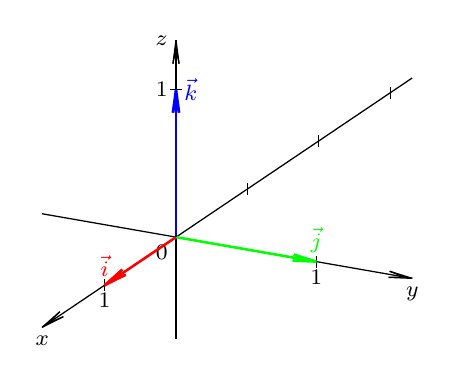
\begin{tikzpicture}
                    % \clip (0,0) rectangle (14.000000,10.000000);
                    {\footnotesize

                    % Drawing 3D Cartesian system
                    \draw (4.000000,4.000000) node [anchor=north east] { $0$ };%
                    \draw [line width=0.016cm] (4.000000,3.925000) -- (4.000000,4.075000);%
                    \draw (3.092808,3.388814) node [anchor=north] { $1$ };%
                    \draw [line width=0.016cm] (3.092808,3.313814) -- (3.092808,3.463814);%
                    % \draw (4.907192,4.611186) node [anchor=north] { $-1$ };%
                    \draw [line width=0.016cm] (4.907192,4.536186) -- (4.907192,4.686186);%
                    % \draw (5.814384,5.222372) node [anchor=north] { $-2$ };%
                    \draw [line width=0.016cm] (5.814384,5.147372) -- (5.814384,5.297372);%
                    % \draw (6.721577,5.833558) node [anchor=north] { $-3$ };%
                    \draw [line width=0.016cm] (6.721577,5.758558) -- (6.721577,5.908558);%
                    \draw (5.782415,3.688926) node [anchor=north] { $1$ };%
                    \draw [line width=0.016cm] (5.782415,3.613926) -- (5.782415,3.763926);%
                    \draw (4.000000,5.878745) node [anchor=east] { $1$ };%
                    \draw [line width=0.016cm] (3.925000,5.878745) -- (4.075000,5.878745);%
                    \draw (2.300000,2.854690) node [anchor=north] { $x$ };%
                    \draw (7.000000,3.476428) node [anchor=north] { $y$ };%
                    \draw (4.000000,6.500000) node [anchor=east] { $z$ };%
                    \draw [line width=0.016cm] (2.300000,2.854690) -- (7.000000,6.021135);%
                    \draw [line width=0.016cm] (2.568554,2.988402) -- (2.300000,2.854690);%
                    \draw [line width=0.016cm] (2.568554,2.988402) -- (2.382934,2.910564);%
                    \draw [line width=0.016cm] (2.524796,3.053353) -- (2.300000,2.854690);%
                    \draw [line width=0.016cm] (2.524796,3.053353) -- (2.382934,2.910564);%
                    \draw [line width=0.016cm] (2.300000,4.296691) -- (7.000000,3.476428);%
                    \draw [line width=0.016cm] (6.713728,3.566139) -- (7.000000,3.476428);%
                    \draw [line width=0.016cm] (6.713728,3.566139) -- (6.901489,3.493620);%
                    \draw [line width=0.016cm] (6.700263,3.488989) -- (7.000000,3.476428);%
                    \draw [line width=0.016cm] (6.700263,3.488989) -- (6.901489,3.493620);%
                    \draw [line width=0.016cm] (4.000000,2.700000) -- (4.000000,6.500000);%
                    \draw [line width=0.016cm] (3.960842,6.202567) -- (4.000000,6.500000);%
                    \draw [line width=0.016cm] (3.960842,6.202567) -- (4.000000,6.400000);%
                    \draw [line width=0.016cm] (4.039158,6.202567) -- (4.000000,6.500000);%
                    \draw [line width=0.016cm] (4.039158,6.202567) -- (4.000000,6.400000);%

                    % Changing color 255 0 0
                    \definecolor{r255g0b0}{rgb}{1.000000,0.000000,0.000000}%
                    \color{r255g0b0}% 

                    % Drawing segment O X
                    \draw [line width=0.032cm] (4.000000,4.000000) -- (3.092808,3.388814);%

                    % Drawing arrow O X 1.00
                    \draw [line width=0.032cm] (3.361361,3.522526) -- (3.092808,3.388814);%
                    \draw [line width=0.032cm] (3.361361,3.522526) -- (3.175033,3.444210);%
                    \draw [line width=0.032cm] (3.317603,3.587477) -- (3.092808,3.388814);%
                    \draw [line width=0.032cm] (3.317603,3.587477) -- (3.175033,3.444210);%

                    % Marking point \vec{i}
                    \draw (3.092808,3.388814) node [anchor=south] { $\vec{i}$ };%

                    % Changing color 0 255 0
                    \definecolor{r0g255b0}{rgb}{0.000000,1.000000,0.000000}%
                    \color{r0g255b0}% 

                    % Drawing segment O Y
                    \draw [line width=0.032cm] (4.000000,4.000000) -- (5.782415,3.688926);%

                    % Drawing arrow O Y 1.00
                    \draw [line width=0.032cm] (5.496142,3.778637) -- (5.782415,3.688926);%
                    \draw [line width=0.032cm] (5.496142,3.778637) -- (5.684746,3.705971);%
                    \draw [line width=0.032cm] (5.482678,3.701487) -- (5.782415,3.688926);%
                    \draw [line width=0.032cm] (5.482678,3.701487) -- (5.684746,3.705971);%

                    % Marking point \vec{j}
                    \draw (5.782415,3.688926) node [anchor=south] { $\vec{j}$ };%

                    % Changing color 0 0 255
                    \definecolor{r0g0b255}{rgb}{0.000000,0.000000,1.000000}%
                    \color{r0g0b255}% 

                    % Drawing segment O Z
                    \draw [line width=0.032cm] (4.000000,4.000000) -- (4.000000,5.878745);%

                    % Drawing arrow O Z 1.00
                    \draw [line width=0.032cm] (3.960842,5.581312) -- (4.000000,5.878745);%
                    \draw [line width=0.032cm] (3.960842,5.581312) -- (4.000000,5.779601);%
                    \draw [line width=0.032cm] (4.039158,5.581312) -- (4.000000,5.878745);%
                    \draw [line width=0.032cm] (4.039158,5.581312) -- (4.000000,5.779601);%

                    % Marking point \vec{k}
                    \draw (4.000000,5.878745) node [anchor=west] { $\vec{k}$ };%
                    \color{black}
                    }
                    \end{tikzpicture}
                    }

            \end{columns}


        \end{frame}


        \begin{frame}
            \frametitle{Krajevni vektor točke}

            \begin{columns}

                \column{0.5\textwidth}

                \only<1->{\begin{alertblock}{}
                    \textbf{Krajevni vektor točke \textcolor{blue}{$T$}} je vektor, ki se začne v koordinatnem izhodišču sistema in konča v točki \textcolor{blue}{$T$}. \\ Označimo ga z \textcolor{red}{\textbf{$\vec{r_T}$}}.
                \end{alertblock}}

                \only<2->{\begin{alertblock}{}
                    \textbf{Komponente krajevnega vektorja \textcolor{red}{$\vec{r_T}$} točke \textcolor{blue}{$T$} so enake koordinatam točke  \textcolor{blue}{$T$}.} $$\textcolor{blue}{T(x_0,y_0,z_0)}$$ $$\textcolor{red}{\vec{r_T}=(x_0,y_0,z_0)}$$
                \end{alertblock}}

                \column{0.48\textwidth}

                \begin{tikzpicture}
                    % \clip (0,0) rectangle (14.000000,10.000000);
                    {\footnotesize
                    
                    % Drawing 3D Cartesian system
                    \draw (4.000000,4.000000) node [anchor=north east] { $0$ };%
                    \draw [line width=0.016cm] (4.000000,3.925000) -- (4.000000,4.075000);%
                    \draw (3.546404,3.694407) node [anchor=north] { $1$ };%
                    \draw [line width=0.016cm] (3.546404,3.619407) -- (3.546404,3.769407);%
                    % \draw (3.092808,3.388814) node [anchor=north] { $2$ };%
                    \draw [line width=0.016cm] (3.092808,3.313814) -- (3.092808,3.463814);%
                    % \draw (2.639212,3.083221) node [anchor=north] { $3$ };%
                    \draw [line width=0.016cm] (2.639212,3.008221) -- (2.639212,3.158221);%
                    % \draw (2.185616,2.777628) node [anchor=north] { $4$ };%
                    \draw [line width=0.016cm] (2.185616,2.702628) -- (2.185616,2.852628);%
                    % \draw (1.732019,2.472035) node [anchor=north] { $5$ };%
                    \draw [line width=0.016cm] (1.732019,2.397035) -- (1.732019,2.547035);%
                    \draw (4.453596,4.305593) node [anchor=north] { $-1$ };%
                    \draw [line width=0.016cm] (4.453596,4.230593) -- (4.453596,4.380593);%
                    % \draw (4.907192,4.611186) node [anchor=north] { $-2$ };%
                    \draw [line width=0.016cm] (4.907192,4.536186) -- (4.907192,4.686186);%
                    % \draw (5.360788,4.916779) node [anchor=north] { $-3$ };%
                    \draw [line width=0.016cm] (5.360788,4.841779) -- (5.360788,4.991779);%
                    % \draw (5.814384,5.222372) node [anchor=north] { $-4$ };%
                    \draw [line width=0.016cm] (5.814384,5.147372) -- (5.814384,5.297372);%
                    % \draw (6.267981,5.527965) node [anchor=north] { $-5$ };%
                    \draw [line width=0.016cm] (6.267981,5.452965) -- (6.267981,5.602965);%
                    % \draw (6.721577,5.833558) node [anchor=north] { $-6$ };%
                    \draw [line width=0.016cm] (6.721577,5.758558) -- (6.721577,5.908558);%
                    % \draw (7.175173,6.139151) node [anchor=north] { $-7$ };%
                    \draw [line width=0.016cm] (7.175173,6.064151) -- (7.175173,6.214151);%
                    \draw (4.891207,3.844463) node [anchor=north] { $1$ };%
                    \draw [line width=0.016cm] (4.891207,3.769463) -- (4.891207,3.919463);%
                    % \draw (5.782415,3.688926) node [anchor=north] { $2$ };%
                    \draw [line width=0.016cm] (5.782415,3.613926) -- (5.782415,3.763926);%
                    % \draw (6.673622,3.533389) node [anchor=north] { $3$ };%
                    \draw [line width=0.016cm] (6.673622,3.458389) -- (6.673622,3.608389);%
                    \draw (3.108793,4.155537) node [anchor=north] { $-1$ };%
                    \draw [line width=0.016cm] (3.108793,4.080537) -- (3.108793,4.230537);%
                    % \draw (2.217585,4.311074) node [anchor=north] { $-2$ };%
                    \draw [line width=0.016cm] (2.217585,4.236074) -- (2.217585,4.386074);%
                    % \draw (1.326378,4.466611) node [anchor=north] { $-3$ };%
                    \draw [line width=0.016cm] (1.326378,4.391611) -- (1.326378,4.541611);%
                    \draw (4.000000,4.939373) node [anchor=east] { $1$ };%
                    \draw [line width=0.016cm] (3.925000,4.939373) -- (4.075000,4.939373);%
                    % \draw (4.000000,5.878745) node [anchor=east] { $2$ };%
                    \draw [line width=0.016cm] (3.925000,5.878745) -- (4.075000,5.878745);%
                    % \draw (4.000000,6.818118) node [anchor=east] { $3$ };%
                    \draw [line width=0.016cm] (3.925000,6.818118) -- (4.075000,6.818118);%
                    \draw (4.000000,3.060627) node [anchor=east] { $-1$ };%
                    \draw [line width=0.016cm] (3.925000,3.060627) -- (4.075000,3.060627);%
                    % \draw (4.000000,2.121255) node [anchor=east] { $-2$ };%
                    \draw [line width=0.016cm] (3.925000,2.121255) -- (4.075000,2.121255);%
                    \draw (1.300000,2.180978) node [anchor=north] { $x$ };%
                    \draw (7.500000,3.389166) node [anchor=north] { $y$ };%
                    \draw (4.000000,7.700000) node [anchor=east] { $z$ };%
                    \draw [line width=0.016cm] (1.300000,2.180978) -- (3.150353,3.427583);%
                    \draw [line width=0.016cm] (3.216701,3.472282) -- (7.500000,6.357991);%
                    \draw [line width=0.016cm] (1.568554,2.314690) -- (1.300000,2.180978);%
                    \draw [line width=0.016cm] (1.568554,2.314690) -- (1.382934,2.236852);%
                    \draw [line width=0.016cm] (1.524796,2.379641) -- (1.300000,2.180978);%
                    \draw [line width=0.016cm] (1.524796,2.379641) -- (1.382934,2.236852);%
                    \draw [line width=0.016cm] (1.300000,4.471215) -- (6.188614,3.618034);%
                    \draw [line width=0.016cm] (6.267423,3.604280) -- (7.500000,3.389166);%
                    \draw [line width=0.016cm] (7.213728,3.478877) -- (7.500000,3.389166);%
                    \draw [line width=0.016cm] (7.213728,3.478877) -- (7.401489,3.406358);%
                    \draw [line width=0.016cm] (7.200263,3.401727) -- (7.500000,3.389166);%
                    \draw [line width=0.016cm] (7.200263,3.401727) -- (7.401489,3.406358);%
                    \draw [line width=0.016cm] (4.000000,1.800000) -- (4.000000,6.308432);%
                    \draw [line width=0.016cm] (4.000000,6.388432) -- (4.000000,7.700000);%
                    \draw [line width=0.016cm] (3.960842,7.402567) -- (4.000000,7.700000);%
                    \draw [line width=0.016cm] (3.960842,7.402567) -- (4.000000,7.600000);%
                    \draw [line width=0.016cm] (4.039158,7.402567) -- (4.000000,7.700000);%
                    \draw [line width=0.016cm] (4.039158,7.402567) -- (4.000000,7.600000);%
                    
                    % Changing color 220 220 220
                    \definecolor{r220g220b220}{rgb}{0.862745,0.862745,0.862745}%
                    \color{r220g220b220}% 
                    
                    % Drawing segment T xy
                    \draw [line width=0.016cm] (5.411545,5.369522) -- (5.411545,5.259522);%
                    \draw [line width=0.016cm] (5.411545,5.184522) -- (5.411545,5.034522);%
                    \draw [line width=0.016cm] (5.411545,4.959522) -- (5.411545,4.809522);%
                    \draw [line width=0.016cm] (5.411545,4.734522) -- (5.411545,4.584522);%
                    \draw [line width=0.016cm] (5.411545,4.509522) -- (5.411545,4.359522);%
                    \draw [line width=0.016cm] (5.411545,4.284522) -- (5.411545,4.134522);%
                    \draw [line width=0.016cm] (5.411545,4.059522) -- (5.411545,3.909522);%
                    \draw [line width=0.016cm] (5.411545,3.834522) -- (5.411545,3.684522);%
                    \draw [line width=0.016cm] (5.411545,3.609522) -- (5.411545,3.459522);%
                    \draw [line width=0.016cm] (5.411545,3.384522) -- (5.411545,3.234522);%
                    \draw [line width=0.016cm] (5.411545,3.159522) -- (5.411545,3.061090);%
                    
                    % Drawing segment xy x
                    \draw [line width=0.016cm] (5.411545,3.061090) -- (5.263779,3.086879);%
                    \draw [line width=0.016cm] (5.189896,3.099773) -- (5.042129,3.125562);%
                    \draw [line width=0.016cm] (4.968246,3.138456) -- (4.820479,3.164245);%
                    \draw [line width=0.016cm] (4.746596,3.177139) -- (4.598830,3.202928);%
                    \draw [line width=0.016cm] (4.524946,3.215823) -- (4.377180,3.241611);%
                    \draw [line width=0.016cm] (4.303297,3.254506) -- (4.155530,3.280295);%
                    \draw [line width=0.016cm] (4.081647,3.293189) -- (3.933880,3.318978);%
                    \draw [line width=0.016cm] (3.859997,3.331872) -- (3.712231,3.357661);%
                    \draw [line width=0.016cm] (3.638347,3.370555) -- (3.490581,3.396344);%
                    \draw [line width=0.016cm] (3.416698,3.409239) -- (3.268931,3.435027);%
                    
                    % Drawing segment xy y
                    \draw [line width=0.016cm] (5.411545,3.061090) -- (5.535947,3.144901);%
                    \draw [line width=0.016cm] (5.598148,3.186806) -- (5.722549,3.270617);%
                    \draw [line width=0.016cm] (5.784750,3.312522) -- (5.909152,3.396333);%
                    \draw [line width=0.016cm] (5.971352,3.438238) -- (6.095754,3.522049);%
                    \draw [line width=0.016cm] (6.157955,3.563955) -- (6.194845,3.588808);%
                    
                    % Drawing segment y yz
                    \draw [line width=0.016cm] (6.228018,3.651157) -- (6.228018,3.761157);%
                    \draw [line width=0.016cm] (6.228018,3.836157) -- (6.228018,3.986157);%
                    \draw [line width=0.016cm] (6.228018,4.061157) -- (6.228018,4.211157);%
                    \draw [line width=0.016cm] (6.228018,4.286157) -- (6.228018,4.436157);%
                    \draw [line width=0.016cm] (6.228018,4.511157) -- (6.228018,4.661157);%
                    \draw [line width=0.016cm] (6.228018,4.736157) -- (6.228018,4.886157);%
                    \draw [line width=0.016cm] (6.228018,4.961157) -- (6.228018,5.111157);%
                    \draw [line width=0.016cm] (6.228018,5.186157) -- (6.228018,5.336157);%
                    \draw [line width=0.016cm] (6.228018,5.411157) -- (6.228018,5.561157);%
                    \draw [line width=0.016cm] (6.228018,5.636157) -- (6.228018,5.786157);%
                    \draw [line width=0.016cm] (6.228018,5.861157) -- (6.228018,5.959589);%
                    
                    % Drawing segment yz z
                    \draw [line width=0.016cm] (6.228018,5.959589) -- (6.080252,5.985378);%
                    \draw [line width=0.016cm] (6.006369,5.998272) -- (5.858602,6.024061);%
                    \draw [line width=0.016cm] (5.784719,6.036955) -- (5.636952,6.062744);%
                    \draw [line width=0.016cm] (5.563069,6.075639) -- (5.415303,6.101427);%
                    \draw [line width=0.016cm] (5.341419,6.114322) -- (5.193653,6.140111);%
                    \draw [line width=0.016cm] (5.119770,6.153005) -- (4.972003,6.178794);%
                    \draw [line width=0.016cm] (4.898120,6.191688) -- (4.750353,6.217477);%
                    \draw [line width=0.016cm] (4.676470,6.230371) -- (4.528704,6.256160);%
                    \draw [line width=0.016cm] (4.454820,6.269055) -- (4.307054,6.294843);%
                    \draw [line width=0.016cm] (4.233171,6.307738) -- (4.085404,6.333527);%
                    
                    % Drawing segment T yz
                    \draw [line width=0.016cm] (5.444719,5.431871) -- (5.535947,5.493332);%
                    \draw [line width=0.016cm] (5.598148,5.535238) -- (5.722549,5.619049);%
                    \draw [line width=0.016cm] (5.784750,5.660954) -- (5.909152,5.744765);%
                    \draw [line width=0.016cm] (5.971352,5.786670) -- (6.095754,5.870481);%
                    \draw [line width=0.016cm] (6.157955,5.912386) -- (6.228018,5.959589);%
                    
                    % Drawing segment T xz
                    \draw [line width=0.016cm] (5.372141,5.416399) -- (5.263779,5.435310);%
                    \draw [line width=0.016cm] (5.189896,5.448205) -- (5.042129,5.473994);%
                    \draw [line width=0.016cm] (4.968246,5.486888) -- (4.820479,5.512677);%
                    \draw [line width=0.016cm] (4.746596,5.525571) -- (4.598830,5.551360);%
                    \draw [line width=0.016cm] (4.524946,5.564254) -- (4.377180,5.590043);%
                    \draw [line width=0.016cm] (4.303297,5.602938) -- (4.155530,5.628726);%
                    \draw [line width=0.016cm] (4.081647,5.641621) -- (3.933880,5.667410);%
                    \draw [line width=0.016cm] (3.859997,5.680304) -- (3.712231,5.706093);%
                    \draw [line width=0.016cm] (3.638347,5.718987) -- (3.490581,5.744776);%
                    \draw [line width=0.016cm] (3.416698,5.757670) -- (3.268931,5.783459);%
                    \draw [line width=0.016cm] (3.195048,5.796354) -- (3.183527,5.798364);%
                    
                    % Drawing segment x xz
                    \draw [line width=0.016cm] (3.183527,3.489933) -- (3.183527,3.599933);%
                    \draw [line width=0.016cm] (3.183527,3.674933) -- (3.183527,3.824933);%
                    \draw [line width=0.016cm] (3.183527,3.899933) -- (3.183527,4.049933);%
                    \draw [line width=0.016cm] (3.183527,4.124933) -- (3.183527,4.274933);%
                    \draw [line width=0.016cm] (3.183527,4.349933) -- (3.183527,4.499933);%
                    \draw [line width=0.016cm] (3.183527,4.574933) -- (3.183527,4.724933);%
                    \draw [line width=0.016cm] (3.183527,4.799933) -- (3.183527,4.949933);%
                    \draw [line width=0.016cm] (3.183527,5.024933) -- (3.183527,5.174933);%
                    \draw [line width=0.016cm] (3.183527,5.249933) -- (3.183527,5.399933);%
                    \draw [line width=0.016cm] (3.183527,5.474933) -- (3.183527,5.624933);%
                    \draw [line width=0.016cm] (3.183527,5.699933) -- (3.183527,5.798364);%
                    
                    % Drawing segment xz z
                    \draw [line width=0.016cm] (3.183527,5.798364) -- (3.307929,5.882175);%
                    \draw [line width=0.016cm] (3.370129,5.924080) -- (3.494531,6.007891);%
                    \draw [line width=0.016cm] (3.556732,6.049797) -- (3.681133,6.133607);%
                    \draw [line width=0.016cm] (3.743334,6.175513) -- (3.867736,6.259324);%
                    \draw [line width=0.016cm] (3.929936,6.301229) -- (3.966826,6.326082);%
                    
                    % Changing color 0 0 0
                    \definecolor{r0g0b0}{rgb}{0.000000,0.000000,0.000000}%
                    \color{r0g0b0}% 
                    
                    % Marking point x by circle
                    \draw [line width=0.016cm] (3.183527,3.449933) circle (0.040000);%
                    
                    % Marking point x_0
                    \draw (3.183527,3.449933) node [anchor=east] { $x_0$ };%
                    
                    % Marking point z by circle
                    \draw [line width=0.016cm] (4.000000,6.348432) circle (0.040000);%
                    
                    % Marking point z_0
                    \draw (4.000000,6.348432) node [anchor=east] { $z_0$ };%
                    
                    % Marking point y by circle
                    \draw [line width=0.016cm] (6.228018,3.611157) circle (0.040000);%
                    
                    % Marking point y_0
                    \draw (6.228018,3.611157) node [anchor=south west] { $y_0$ };%
                    
                    % Changing color 0 0 255
                    \definecolor{r0g0b255}{rgb}{0.000000,0.000000,1.000000}%
                    \color{r0g0b255}% 
                    
                    % Marking point T by circle
                    \draw [line width=0.032cm] (5.411545,5.409522) circle (0.040000);%
                    \only<1>{\draw (5.241545,5.379522) node [anchor=south west] { $T$ };}%            
                    \only<2->{\draw (5.241545,5.379522) node [anchor=south west] { $T(x_0,y_0,z_0)$ };}%

                    % Changing color 255 0 0
                    \definecolor{r255g0b0}{rgb}{1.000000,0.000000,0.000000}%
                    \color{r255g0b0}% 
                    
                    % Drawing segment O T
                    \draw [line width=0.032cm] (4.000000,4.000000) -- (5.383241,5.381258);%
                    
                    % Drawing arrow O T 1.00
                    \draw [line width=0.032cm] (5.173408,5.227064) -- (5.379794,5.385194);%
                    \draw [line width=0.032cm] (5.173408,5.227064) -- (5.341389,5.339466);%
                    \draw [line width=0.032cm] (5.228746,5.171647) -- (5.387172,5.377805);%
                    \draw [line width=0.032cm] (5.228746,5.171647) -- (5.341389,5.339466);%
                    
                    % Changing color 255 0 0
                    \definecolor{r255g0b0}{rgb}{1.000000,0.000000,0.000000}%
                    \color{r255g0b0}% 
                    
                    % Marking point \vec{r_T}
                    \only<1>{\draw (5.111545,5.239835) node [anchor=north west] { $\vec{r_T}$ };}%
                    \only<2->{\draw (5.111545,5.239835) node [anchor=north west] { $\vec{r_T}=(x_0,y_0,z_0)$ };}%

                    \color{black}
                    }
                    \end{tikzpicture}
                

            \end{columns}
        \end{frame}

        \begin{frame}
            
            \only<2->{\begin{alertblock}{}
                Tudi standardne bazne vektorje $\vec{i}$, $\vec{j}$ in $\vec{k}$ lahko zapišemo kot krajevne vektorje:
                $\vec{i}=(1,0,0)$, $\vec{j}=(0,1,0)$ in $\vec{k}=(0,0,1)$.
            \end{alertblock}}

            \only<3->{\begin{alertblock}{}
                Poljuben vektor $\vec{v}$ v prostoru lahko zapišemo kot linearno kombinacijo standardnih baznih vektorjev:
                $$\vec{v}=\alpha\vec{i}+\beta\vec{j}+\gamma\vec{k}=(\alpha,\beta,\gamma)$$
            \end{alertblock}}

            \begin{columns}
                \column{0.5\textwidth}
                    \only<4->{\begin{alertblock}{}
                        S krajevnimi vektorji lahko izrazimo poljuben vektor \textcolor{red}{$\vec{AB}$}, z začetkom v točki $A$ in koncem v točki $B$:
                        \only<5->{$$\textcolor{red}{\vec{AB}}=\textcolor{gray}{\vec{r_B}-\vec{r_A}}$$}
                    \end{alertblock}}

                \column{0.48\textwidth}

                \only<4->{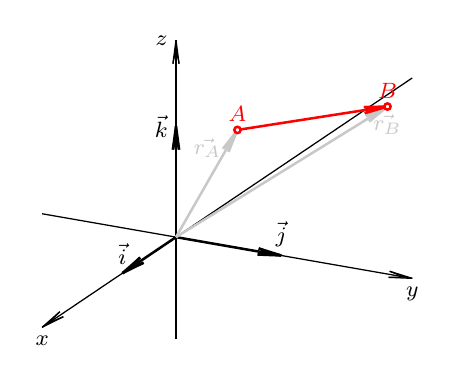
\begin{tikzpicture}
                    % \clip (0,0) rectangle (14.000000,10.000000);
                    {\footnotesize
                    
                    % Drawing 3D Cartesian system
                    \draw (2.300000,2.854690) node [anchor=north] { $x$ };%
                    \draw (7.000000,3.476428) node [anchor=north] { $y$ };%
                    \draw (4.000000,6.500000) node [anchor=east] { $z$ };%
                    \draw [line width=0.016cm] (2.300000,2.854690) -- (7.000000,6.021135);%
                    \draw [line width=0.016cm] (2.568554,2.988402) -- (2.300000,2.854690);%
                    \draw [line width=0.016cm] (2.568554,2.988402) -- (2.382934,2.910564);%
                    \draw [line width=0.016cm] (2.524796,3.053353) -- (2.300000,2.854690);%
                    \draw [line width=0.016cm] (2.524796,3.053353) -- (2.382934,2.910564);%
                    \draw [line width=0.016cm] (2.300000,4.296691) -- (7.000000,3.476428);%
                    \draw [line width=0.016cm] (6.713728,3.566139) -- (7.000000,3.476428);%
                    \draw [line width=0.016cm] (6.713728,3.566139) -- (6.901489,3.493620);%
                    \draw [line width=0.016cm] (6.700263,3.488989) -- (7.000000,3.476428);%
                    \draw [line width=0.016cm] (6.700263,3.488989) -- (6.901489,3.493620);%
                    \draw [line width=0.016cm] (4.000000,2.700000) -- (4.000000,6.500000);%
                    \draw [line width=0.016cm] (3.960842,6.202567) -- (4.000000,6.500000);%
                    \draw [line width=0.016cm] (3.960842,6.202567) -- (4.000000,6.400000);%
                    \draw [line width=0.016cm] (4.039158,6.202567) -- (4.000000,6.500000);%
                    \draw [line width=0.016cm] (4.039158,6.202567) -- (4.000000,6.400000);%
                    
                    % Drawing segment O X
                    \draw [line width=0.032cm] (4.000000,4.000000) -- (3.319606,3.541610);%
                    
                    % Drawing arrow O X 1.00
                    \draw [line width=0.032cm] (3.588159,3.675323) -- (3.319606,3.541610);%
                    \draw [line width=0.032cm] (3.588159,3.675323) -- (3.401831,3.597006);%
                    \draw [line width=0.032cm] (3.544401,3.740273) -- (3.319606,3.541610);%
                    \draw [line width=0.032cm] (3.544401,3.740273) -- (3.401831,3.597006);%
                    
                    % Marking point \vec{i}
                    \draw (3.319606,3.541610) node [anchor=south] { $\vec{i}$ };%
                    
                    % Drawing segment O Y
                    \draw [line width=0.032cm] (4.000000,4.000000) -- (5.336811,3.766694);%
                    
                    % Drawing arrow O Y 1.00
                    \draw [line width=0.032cm] (5.050539,3.856405) -- (5.336811,3.766694);%
                    \draw [line width=0.032cm] (5.050539,3.856405) -- (5.239143,3.783740);%
                    \draw [line width=0.032cm] (5.037074,3.779256) -- (5.336811,3.766694);%
                    \draw [line width=0.032cm] (5.037074,3.779256) -- (5.239143,3.783740);%
                    
                    % Marking point \vec{j}
                    \draw (5.336811,3.766694) node [anchor=south] { $\vec{j}$ };%
                    
                    % Drawing segment O Z
                    \draw [line width=0.032cm] (4.000000,4.000000) -- (4.000000,5.409059);%
                    
                    % Drawing arrow O Z 1.00
                    \draw [line width=0.032cm] (3.960842,5.111626) -- (4.000000,5.409059);%
                    \draw [line width=0.032cm] (3.960842,5.111626) -- (4.000000,5.309915);%
                    \draw [line width=0.032cm] (4.039158,5.111626) -- (4.000000,5.409059);%
                    \draw [line width=0.032cm] (4.039158,5.111626) -- (4.000000,5.309915);%
                    
                    % Marking point \vec{k}
                    \draw (4.000000,5.409059) node [anchor=east] { $\vec{k}$ };%
                    
                    % Changing color 200 200 200
                    \definecolor{r200g200b200}{rgb}{0.784314,0.784314,0.784314}%
                    \color{r200g200b200}% 
                    
                    % Drawing segment O A
                    \draw [line width=0.032cm] (4.000000,4.000000) -- (4.760611,5.326546);%
                    
                    % Drawing segment O B
                    \draw [line width=0.032cm] (4.000000,4.000000) -- (6.651577,5.637380);%
                    
                    % Drawing arrow O A 1.00
                    \draw [line width=0.032cm] (4.598590,5.122696) -- (4.756251,5.329440);%
                    \draw [line width=0.032cm] (4.598590,5.122696) -- (4.731191,5.275237);%
                    \draw [line width=0.032cm] (4.666530,5.083741) -- (4.765310,5.324246);%
                    \draw [line width=0.032cm] (4.666530,5.083741) -- (4.731191,5.275237);%
                    
                    % Drawing arrow O B 1.00
                    \draw [line width=0.032cm] (6.411966,5.535439) -- (6.649125,5.642002);%
                    \draw [line width=0.032cm] (6.411966,5.535439) -- (6.601254,5.606305);%
                    \draw [line width=0.032cm] (6.453114,5.468804) -- (6.654611,5.633117);%
                    \draw [line width=0.032cm] (6.453114,5.468804) -- (6.601254,5.606305);%
                    
                    % Marking point \vec{r_A}
                    \draw (4.680507,5.361247) node [anchor=north east] { $\vec{r_A}$ };%
                    
                    % Marking point \vec{r_B}
                    \draw (6.685611,5.658396) node [anchor=north] { $\vec{r_B}$ };%
                    
                    % Changing color 255 0 0
                    \definecolor{r255g0b0}{rgb}{1.000000,0.000000,0.000000}%
                    \color{r255g0b0}% 
                    
                    % Marking point A by circle
                    \draw [line width=0.032cm] (4.780507,5.361247) circle (0.040000);%
                    \draw (4.780507,5.361247) node [anchor=south] { $A$ };%
                    
                    % Marking point B by circle
                    \draw [line width=0.032cm] (6.685611,5.658396) circle (0.040000);%
                    \draw (6.685611,5.658396) node [anchor=south] { $B$ };%
                    
                    % Drawing segment A B
                    \draw [line width=0.032cm] (4.820029,5.367411) -- (6.646089,5.652232);%
                    
                    % Drawing arrow A B 1.00
                    \draw [line width=0.032cm] (6.385696,5.651248) -- (6.645622,5.657443);%
                    \draw [line width=0.032cm] (6.385696,5.651248) -- (6.587651,5.643117);%
                    \draw [line width=0.032cm] (6.397765,5.573868) -- (6.647231,5.647126);%
                    \draw [line width=0.032cm] (6.397765,5.573868) -- (6.587651,5.643117);%
                    \color{black}
                    }
                    \end{tikzpicture}}
                    
            \end{columns}


        \end{frame}

        \begin{frame}
            \frametitle{Računanje s krajevnimi vektorji}

            \only<2->{\begin{alertblock}{Seštevanje in odštevanje}
                \only<3->{$$(a_1,a_2,a_3)+(b_1,b_2,b_3)=(a_1+b_1,a_2+b_2,a_3+b_3)$$ }              
                \only<4->{$$(a_1,a_2,a_3)-(b_1,b_2,b_3)=(a_1-b_1,a_2-b_2,a_3-b_3)$$}
            \end{alertblock}}


            \only<5->{\begin{alertblock}{Množenje s skalarjem}
                \only<6->{$$n(a_1,a_2,a_3)=(na_1,na_2,na_3)$$}
            \end{alertblock}}

            \only<7->{\begin{alertblock}{Skalarno množenje}
                \only<8->{$$(a_1,a_2,a_3)(b_1,b_2,b_3)=a_1b_1+a_2b_2+a_3b_3$$}
            \end{alertblock}}
            

            \only<9->{\begin{alertblock}{}
                $$\vec{a}=\vec{b} \Leftrightarrow a_1=b_1 \wedge a_2=b_2 \wedge a_3=b_3$$
            \end{alertblock}}
        \end{frame}

    \subsection{Skalarni produkt v koordinatnem sistemu}

        \begin{frame}
            \frametitle{Skalarni produkt v koordinatnem sistemu}
        \end{frame}

    \subsection{(i) Vektorski produkt}

        \begin{frame}
            \frametitle{(i) Vektorski produkt}
        \end{frame}

    \subsection{(i) Premice v prostoru}

        \begin{frame}
            \frametitle{(i) Premice v prostoru}
        \end{frame}

    \subsection{(i) Ravnine v prostoru}

        \begin{frame}
            \frametitle{(i) Ravnine v prostoru}
        \end{frame}
